\section{Introduction}\label{sec:intro}

Theorem~1 of \cite{OAI} gives one deterministic Turing machine, with a fixed finite alphabet and a fixed finite number of one-dimensional tapes, that multiplies two $n$-bit integers in time
\[
  T(n) = O\bigl(n(\lgn)^{1-\kappa}\bigr), \qquad \kappa = 2^{-182}.
\]
The constants in \cite[\S9.1]{OAI} are chosen ``deliberately conservative; no optimization is claimed''. This note asks how large $\kappa$ can be made while keeping the algorithm's architecture: the motif networks of \cite[\S3]{OAI}, the power-width interchange of \cite[Prop.~11]{OAI}, the simultaneous butterfly layers of \cite[Prop.~14]{OAI}, and the cost accounting of \cite[\S9]{OAI}.

\begin{theorem}[computer-assisted]\label{thm:main}
With the modifications of Sections~\ref{sec:outside} and~\ref{sec:bit}, the algorithm of \cite{OAI} runs in time $O(n(\lgn)^{1-\kappa})$ for every fixed $\kappa < 2^{-58.329}$. Following the convention of \cite[\S9.8]{OAI}, which takes $\kappa = \tfrac12\min_i g_i$ to leave explicit slack for fixed powers of $\log p$, this gives
\[
  \kappa = 2^{-59.335}.
\]
\end{theorem}

\paragraph{Status.} Theorem~\ref{thm:main} is supported by a proof outline (this note and the research notes in the repository \cite{repo}) together with exact machine verification of every numerical condition and gate-level checks of the new network for small parameters. It has not been refereed. The changes alter several procedures of \cite{OAI}, not only its constants. A complete proof would need a careful written argument for each change; Section~\ref{sec:status} lists precisely what is machine-checked and what is not.

\paragraph{Where the gain comes from.} Section~\ref{sec:accounting} shows that once the constants are re-tuned, $\kappa$ is determined almost entirely by one number: the saving exponent $\theta_b = 1-\tau$ of the \emph{bit} motif network, through $\kappa \approx \varepsilon\theta_b^2/2$ with $\varepsilon < 1/5$. The paper's bit network on $h = 100$ points has $\theta_b \approx 2^{-39.7}$; our final network has $\theta_b = 2^{-28.004}$. The improvement is staged as a sequence of packages, each adding to the previous one (Table~\ref{tab:packages}).

\begin{table}[ht]
\centering
\small
\begin{tabularx}{\textwidth}{@{}l l l l X@{}}
\toprule
Pkg & $\kappa$ & $\theta_b = 1-\tau$ & bit stages & change \\
\midrule
paper & $2^{-182}$ & --- & $h=100$ & published constants \\
A3 & $2^{-109.084}$ & $2^{-35.693}$ & 46 & re-tuned free constants (bit $h = 46$, complex $h = 25$) \\
B & $2^{-76.199}$ & $2^{-35.693}$ & 46 & axis exposure by $O(d)$ non-adjacent interchanges; guard $C_1 = 14$ \\
C & $2^{-74.978}$ & $2^{-35.693}$ & 46 & $\delta = 2^{-20}$; $\varepsilon < 1/4$; guard depth with leaf size $d^\beta$ \\
D & $2^{-73.733}$ & $2^{-35.071}$ & $(48,42,48)$ & per-stage designs; stage-1 scratch reused in stage 3 \\
E & $2^{-73.473}$ & $2^{-35.071}$ & $(48,42,48)$ & $\alpha = \lceil (8dp)^{1/4}\rceil$; $\varepsilon < 1/5$ \\
F & $2^{-70.142}$ & $2^{-33.407}$ & $(48,44,48)$ & grouped side-wire gates (sunflowers) \\
G & $2^{-68.616}$ & $2^{-32.644}$ & $(49,43,49)$ & laminar tree groups \\
H & $2^{-61.114}$ & $2^{-28.894}$ & $(51,48,51)$ & side rectangles fed by copy wires \\
I & $2^{-60.017}$ & $2^{-28.345}$ & $(51,50,51)$ & sorted-pattern rectangle cover \\
J & $2^{-59.591}$ & $2^{-28.130}$ & $(51,50,51)$ & copy chains shared across kernels \\
\textbf{K} & $\mathbf{2^{-59.335}}$ & $\mathbf{2^{-28.004}}$ & $(51,50,51)$ & cyclic per-kernel point orders \\
\bottomrule
\end{tabularx}
\caption{Verified packages. Every row is the exact output of \texttt{verification/scripts/verify.py}; each printed ``all constraints hold''.}
\label{tab:packages}
\end{table}

\begin{figure}[ht]
\centering
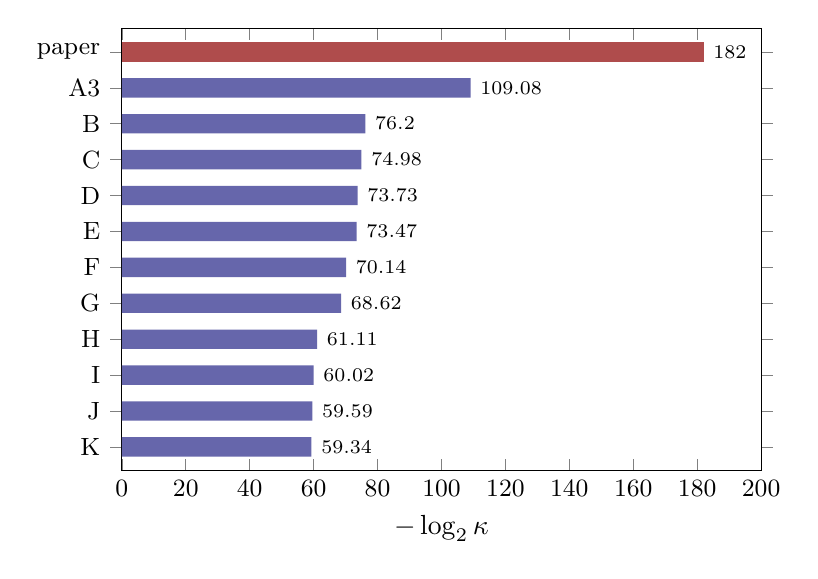
\begin{tikzpicture}
\begin{axis}[
  xbar, bar shift=0pt, width=0.8\textwidth, height=7.2cm,
  xmin=0, xmax=200,
  xlabel={$-\log_2 \kappa$},
  symbolic y coords={K,J,I,H,G,F,E,D,C,B,A3,paper},
  ytick={K,J,I,H,G,F,E,D,C,B,A3,paper}, y dir=normal,
  bar width=7pt,
  nodes near coords, nodes near coords align={horizontal},
  every node near coord/.append style={font=\scriptsize},
  enlarge y limits=0.06,
  tick label style={font=\small},
]
\addplot[fill=blue!45!black!60, draw=none] coordinates {
  (59.335,K) (59.591,J) (60.017,I) (61.114,H) (68.616,G) (70.142,F)
  (73.473,E) (73.733,D) (74.978,C) (76.199,B) (109.084,A3)
};
\addplot[fill=red!55!black!70, draw=none] coordinates {(182,paper)};
\end{axis}
\end{tikzpicture}

\caption{$-\log_2\kappa$ per package (shorter is better).}
\label{fig:bars}
\end{figure}

\paragraph{Lean.} No Lean formalization of \cite{OAI} exists in the OpenAI repository. The statement appears on the Lean FRO evaluation site \cite{LeanEval}. Nothing in this note is formalized.

\paragraph{Organization.} Section~\ref{sec:accounting} recalls the cost table and the rank condition and explains why $\theta_b$ binds. Section~\ref{sec:outside} describes the changes outside the bit network. Section~\ref{sec:bit} describes the new bit network. Section~\ref{sec:verification} describes the verification, Section~\ref{sec:limits} the structural limits and negative results, and Section~\ref{sec:status} the status of each claim.
